\chapter{Aplicația practică}
\label{chap:ch6}

\section{Specificație}
\label{chap:ch6sec1}
\indent \par Aplicația furnizată are rolul de a crea conferințe la care pot participa un număr teoretic nelimitat de participanți. Se pot crea mai multe camere de conferințe (room-uri). Prima persoană care se alătură camerei va fi transmițătorul, iar următorii sunt telespectatorii. 
\indent \par Pentru partea de client, am folosit framework-ul React, profitând de faptul că vine cu un mecanism de \textit{hooks}, prin care se pot reține stările variabilelor (create cu funcția \textit{useState}), în așa fel încât se poate reactualiza o parte din interfață sau toată, în funcție de context. Folosește componente funcționale, putând înlocui cu ușurință implementarea folosind clase. Pentru efectele ulterioare asupra componentei, există un \textit{hook} special numit \textit{useEffect}, la care se poate adăuga un \textit{dependency list}, prin care se specifică variabilele la care se urmărește modificarea valorilor, oricare din ele inițiind o apelare a efectului.
\indent \par Pentru partea de server, am folosit Node.js împreună cu framework-ul \textit{socket.io}, pentru o implementare mai ușoară a mesajelor pe bază de WebSocket. Serverul are rolul de signaling: de a primi cererile de la client de alăturare și de eliminare, dar și de a realiza schimbul de informații necesar pentru a putea realiza transmisia multimedia.
\indent \par Aplicația, așadar, conține următoarele funcționalități:
\begin{enumerate}
    \item Alăturare la o cameră:
    \begin{itemize}
        \item ca transmițător, dacă utilizatorul este primul alăturat
        \item ca telespectator, dacă este oricare din următorii
    \end{itemize}
    \item Comutare între dispozitivele de intrare audio-video (camere web fizice/virtuale, microfoane)
\end{enumerate}
\begin{figure}[!htbp]
    \centering
    \includegraphics[width=12cm]{figures/app_use_case_diagram.png}
    \caption{Diagrama cazurilor de utilizare}
\end{figure}

\section{Design}
\label{chap:ch6sec2}
\begin{figure}[!htbp]
    \centering
    \scalebox{0.65}{\input{figures/app_linked_topology.pdf_tex}}
    \caption{Topologia înlănțuită folosită de fiecare cameră de pe server}
    \label{AppTopology}
\end{figure}
\indent \par În capitolele anterioare, am discutat despre avantajele și dezavantajele fiecărui tip de topologie în cadrul sesiunilor WebRTC. Am descoperit că o topologie mesh aduce avantajul costurilor de întreținere mai mici, datorită lipsei necesității unui server, dar cu compromisul consumului de resurse ridicat pe fiecare nod. De asemenea, serverele media, datorită centralizării locului de transmisie pentru fiecare nod, aduc avantajul ocupării unei lățimi reduse de bandă, ceea ce permite o compresie redusă a imaginii și a sunetului.
\indent \par Există situații în care latența nu este importantă și unde predomină o singură cameră web pornită, unde participanții nu sunt interactivi. Acestea includ: piesele de teatru, concertele, conferințele de lansare a unui produs. În aceste cazuri, vorbim de un scenariu numit broadcasting. Realizat într-o manieră mesh (unul către toți), ar fi ineficient din punct de vedere al resurselor utilizate și a lățimii de bandă, chiar dacă latența este redusă.
\indent \par Pentru aceasta, în aplicația implementată de mine, fiecare cameră reprezintă o topologie de tip lanț, în care nodurile din capete au un singur vecin, iar restul câte doi. Transmisia se va începe de la un capăt și se va termina la celălalt.
\indent \par Diagrama \ref{AppTopology} nu ne dă informații legate de calitatea conexiunii fiecărui client, așadar conexiunile trebuie evaluate. O modalitate simplă este de a testa viteza de descărcare a unui fișier de dimensiuni suficient de mari încât să se descarce rapid pe conexiunile bune. Pentru conexiunile slabe, nu are rost să așteptăm mai mult de 4 secunde, deoarece alăturarea la o cameră va dura mult în acest caz. Un algoritm simplu în JavaScript ar arăta astfel:
\begin{lstlisting}
export const getAverageDownloadSpeed = async () => new Promise((resolve, reject) => {
    const formData = new FormData()
    formData.append('filetype', 'mp3')
    formData.append('filename', 'test')
    formData.append('filesize', 10485760)
  
    let count = 0
    let sum = 0
    let previousDownloadedAmount = 0
    let previousTime = Date.now()
    const request = new XMLHttpRequest()
    request.onprogress = e => {
      const time = Date.now()
      count++
      sum += (e.loaded - previousDownloadedAmount) / (time - previousTime)
      previousDownloadedAmount = e.loaded
      previousTime = time
    }
    const ultimate = setTimeout(() => {
      request.abort()
      resolve(sum / count)
    }, 4000)
  
    request.open('POST', 'https://cors-anywhere.herokuapp.com/https://www.fakefilegenerator.com/download.php')
    request.send(formData)
    request.onreadystatechange = function () {
      if (request.readyState === 4) {
        if (request.status && request.status !== 200) {
          reject(new Error('Request to https://www.fakefilegenerator.com/download.php returned ' + request.status))
        }
        clearTimeout(ultimate)
        resolve(sum / count)
      }
    }
  })
\end{lstlisting}
\indent \par De observat este funcția \texttt{onprogress} din XMLHttpRequest. Aceasta are rolul de a semnala un progres în returnarea datelor de la cerere. Conține un parametru de tip obiect ce va conține câmpurile \textit{loaded} și \textit{total}. Noi vom avea nevoie de câmpul \textit{loaded} pentru a observa cantitatea descărcată la momentul respectiv. Folosind variabile pentru valorile anterioare atât de cantitate, cât și de timp, vom calcula viteza cu care s-a descărcat porțiunea respectivă. Media acestor viteze va fi returnată de către promise. 
\indent \par Vom folosi un timeout pentru o funcție care va returna forțat media vitezelor în cele 4 secunde scurse, în cazul în care nu se finalizează request-ul HTTPS în timp util. Se va reține în variabila \texttt{ultimate} și va fi eliminat în cazul în care request-ul se termină mai repede.
\indent \par Prima dată, după cum am zis, se va alătura transmițătorul la cameră. El va trimite la server mesajul \texttt{[request]rtc:room:join}. Lui i se va crea în memorie un room nou, o topologie nouă și un nod nou (instanță de RTCClientNode). UUID-ul (universally unique identifier) generat de server la conectare va fi ID-ul transmițătorului, urmând ca să primească răspunsul \texttt{[response]rtc:joining-as-broadcaster}.
\begin{figure}[H]
    \centering
    \scalebox{0.7}{\input{figures/app_two_peer_connection.pdf_tex}}
    \caption{Diagrama de secvență pentru conectarea a doi clienți}
\end{figure}
\indent \par Vom adăuga nodurile în topologie în ordinea descrescătoare a acestor viteze de descărcare. Însă schimbul de descriptori SDP dintre cei doi vecini actuali se va anula. Serverul de signaling va fi responsabil de a trimite event-ul \texttt{[webrtc]remove-peer} părintelui noului nod pentru a putea adăuga ulterior track-urile audio-video la acesta. Va șterge track-urile către vechiul său fiu, pentru a nu adăuga același track de două ori, aruncând excepție din cauză că track-ul este deja asociat unui sender RTP de date. Va trimite \texttt{[webrtc]make-offer} pentru ca părintele să facă schimb de SDP-uri cu noul fiu, urmând ca fiul, după ce primește minim două track-uri (se consideră că unul e audio și celălalt e video), să interogheze serverul pentru noii săi fii, pe care îi va adăuga îl lista sa reținută local. Va aștepta două track-uri de la părinte, deoarece, altfel, lista de track-uri ar fi incompletă, necesitând un alt schimb de descriptori.
\begin{figure}[H]
    \centering
    \scalebox{0.7}{\input{figures/app_three_peer_connection.pdf_tex}}
    \caption{Diagrama de secvență pentru conectarea a trei clienți}
\end{figure}
\indent \par Schimbul imaginii de la cameră presupune trimiterea de noi track-uri către toți clienții. Este bine de știut că RTCPeerConnection va apela funcția \textit{onnegotiationneeded} la fiecare track scos. Dar folosirea acestei funcții va complica implementarea. Așadar, se vor scoate, mai întâi, toate track-urile către fiu și se va trimite \texttt{[webrtc]send-offer} pentru a forța schimbul de descriptori. Fiul său va trimite, de asemenea, aceeași cerere către fiul său, până când toți fiii vor primi noile track-uri de la broadcaster.
\indent \par Din motive de stabilitate, trebuie tratat și cazul când un client va părăsi camera, fie apăsând un buton de părăsire, fie închizând forțat pagina web. Părintele său va fi semnalat că trebuie să îl elimine din lista sa de vecini, urmând ca serverul să îi trimită cereri de tip \texttt{[webrtc]make-offer} către fiecare fiu al său. Apoi, se va parcurge pe server topologia înlănțuită și se va căuta după UUID-ul său, eliminându-l și legând vecinii între ei și la nivel logic.
\indent \par Diagrama de clase va arăta în felul următor:
\begin{figure}[H]
    \centering
    \includegraphics[width=15cm]{figures/app_class_diagram.png}
    \caption{Diagrama de clase a aplicației server}
\end{figure}
\indent \par Se vor folosi și variabile de mediu pentru a reține parametrii necesari:
\begin{itemize}
    \item \textbf{PORT} - portul care va fi deschis pentru ascultarea cererilor;
    \item \textbf{CLIENT\_TOPOLOGY} - topologia care va fi folosită (în acest caz, va fi \textit{list}).
\end{itemize}
\indent \par Pe aplicația clientului, clasa care încapsulează logica menționată mai sus este RTCForwardingPeer. Ea va asculta după toate evenimentele primite de la server și va acționa conform. Include câteva event handlere: pentru schimbarea stării conexiunii WebSocket (inițial va fi \textit{disconnected}, urmând să fie \textit{connected}); pentru primirea unei cereri noi de la nodul părinte (\textit{onParentOffer}), care va fi folosit pentru a opri stream-ul din elementul \textit{video} din componenta VideoBroadcastItem; dar și pentru anunțarea sosirea unui track nou de la părinte, \textit{onTrack}, care va porni redarea stream-ului din elementul \textit{video} menționat anterior.
\indent \par Această clasă va fi îmbrăcată sub formă de hook-uri React în componenta \textit{useWebRTC}. Va fi reactualizată în momentul în care se va schimba room-ul în care va participa, dar și în momentul în care se schimbă starea conexiunii cu serverul.
\begin{figure}[H]
    \centering
    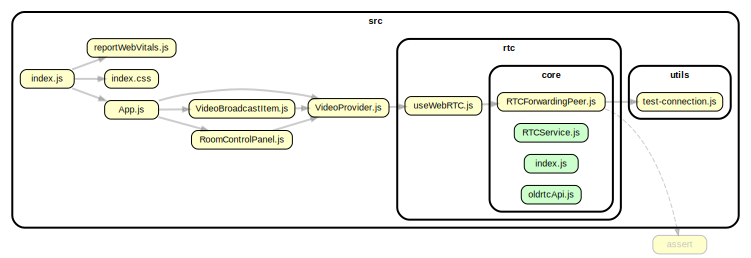
\includegraphics[width=15cm]{figures/app_frontend_dependency_diagram.png}
    \caption{Diagrama de dependințe a aplicației client}
\end{figure}
\section{Utilizare și testare}
\indent \par Utilizatorul, când va deschide aplicația, va fi întâmpinat de această pagină:
\begin{figure}[H]
    \centering
    \includegraphics[width=6.5cm]{figures/app_welcome_screen.png}
    \caption{Ecranul principal}
\end{figure}
\indent \par După ce tastează numele unei camere și va apăsa pe butonul \textit{Join room}, va fi întâmpinat cu unul din cele două ecrane:
\begin{figure}[H]
    \centering
    \begin{subfigure}{0.45\textwidth}
        \centering
        \includegraphics[width=8cm, height=5.5cm]{figures/app_broadcaster_mode.png}
        \caption{Ecranul transmițătorului}
    \end{subfigure}
    \hfill
    \begin{subfigure}{0.45\textwidth}
        \centering
        \includegraphics[width=8cm, height=5.5cm]{figures/app_viewer_mode.png}
        \caption{Ecranul spectatorului}
    \end{subfigure}
\end{figure}
\indent \par Transmițătorul poate comuta între camerele web dând click pe meniul cu opțiuni de sub textul \textit{Choose a camera}:
\begin{figure}[H]
    \centering
    \includegraphics[width=7cm]{figures/app_pick_camera.png}
    \caption{Meniul ce conține lista disponibilă de camere}
\end{figure}
\indent \par Pentru a putea observa lățimea de bandă disponibilă, am afișat în consolă viteza obținută la test. Pe o conexiune pe fir de la Vodafone cu viteză maximă de download de 300 Mbps, am obținut următoarele rezultate:
\begin{figure}[H]
    \centering
    \includegraphics[width=12cm]{figures/app_bandwidth_test.png}
    \caption{Test de lățime de bandă cu rezultatul afișat în consolă (viteza este afișată în KB/s)}
\end{figure}
\begin{figure}[H]
    \centering
    \includegraphics[width=12cm]{figures/app_bandwidth_test_2.png}
    \caption{Al doilea test de lățime de bandă cu rezultatul afișat în consolă}
\end{figure}
\indent \par Am realizat testarea și pe 3 browsere diferite, printre care unul rulând de pe o mașină virtuală cu Linux aflată pe un alt computer. Între transmițător (Microsoft Edge) și Firefox pe Windows, latența observată era minimă, datorită faptului că au rulat pe aceeași mașină, așadar folosind candidații ICE de tip host. Pe Linux, latența era vizibilă.
\indent \par La al doilea test cu același set de browsere, am obținut de la Edge viteza de 127.7740961 KB/s, de la Firefox de pe Linux 606.08179903 KB/s, iar de la cel rulat local pe Windows 258.1044269. Latența imaginii a fost mare pe instanța locală de Firefox, datorită drumului lung care trece prin mașina virtuală. Însă calitatea s-a păstrat identică.
\begin{figure}[H]
    \centering
    \includegraphics[width=12cm]{figures/app_on_3_browsers.png}
    \caption{Aplicația testată pe 3 browsere diferite: Microsoft Edge pe Windows, Mozilla Firefox pe Windows și Mozilla Firefox pe Linux}
\end{figure}
\indent \par Se poate ține cont și de geolocație, precum și de faptul dacă un spectator se află pe aceeași rețea cu transmițătorul, însă acestea vor fi considerate îmbunătățiri pentru viitor.